\addcontentsline{toc}{chapter}{Introduzione}
\chapter*{Introduzione}
Il \textit{Machine Learning}, detto anche Apprendimento Automatico, nasce come diramazione dell'intelligenza artificiale e trova  campi di applicazione sempre più ampi nel mondo contemporaneo.  
In passato questa disciplina era limitata dall'hardware disponibile ma ora, grazie all'avvento di \ac{gpu} sempre più potenti o addirittura hardware dedicato, riusciamo ad usare modelli sempre più complessi e precisi in diversi ambiti della vita quotidiana. 

Il trend attuale prevede l'utilizzo sempre maggiore di Reti Neurali artificiali. Una Rete Neurale è un modello matematico che per molti versi cerca di ricalcare la funzionalità 
di un cervello umano allo scopo di sostituirlo per quei compiti che possono essere definiti \textit{ripetitivi}. 

Il cervello umano è composto da neuroni connessi tra di loro che formano una rete, uno di questi componenti è schematizzato sinteticamente in Figura \ref{fig:neurone}. 
\begin{figure}[]
    \centering
    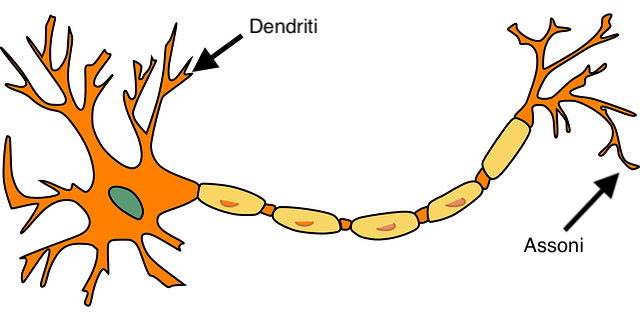
\includegraphics[width = \textwidth]{images/neurone.png}
    \caption{Schema di un neurone}
    \label{fig:neurone}
\end{figure}
All'interno di un neurone gli impulsi elettrici scorrono fino ad arrivare dall'assone, dopodiché sono modulati dalle sinapsi ed infine arrivano ai dendriti degli altri neuroni connessi ad esso formando una rete.

Una rete neurale artificiale prende come modello il cervello umano quindi è composta da tanti neuroni artificiali analoghi ad un neurone biologico; essi ricevono in input dei dati che vengono 
modulati da dei \textit{pesi} ed infine passando per una \textit{funzione di attivazione} vengono restituiti in output ad altri neuroni artificiali. 

Un esempio di utilizzo può essere la guida autonoma: molte case costruttrici, integrando hardware molto potente in situazioni critiche, riescono ad  adottare reti neurali per realizzare veicoli sempre più sicuri e per ridurre l'intervento umano in casi di emergenza o durante lunghi viaggi. 
Lo stato dell'arte in ambito consumer sulla guida autonoma è stato raggiunto dall'americana \textit{Tesla} con il suo \textit{AutoPilot} che, 
grazie a nove telecamere posizionate attorno alla vettura, riesce a raggiungere un livello di autonomia mai visto prima.
Altri utilizzi possono essere la videosorveglianza, dove riconoscere intrusioni di persone o vetture all'interno di un perimetro diventa un compito critico e molto importante che fino a pochi anni fa era prerogativa esclusiva di esseri umani. 
Le reti neurali sono usate anche per controllo qualità, \textit{speech recognition}, \textit{sentiment analysis} e per vari altri compiti. 


Il nostro interesse sarà focalizzato sul miglioramento del riconoscimento di oggetti su immagini rilevate nello spettro termico in quanto offrono un vantaggio in condizioni di scarsa visibilità rispetto alle immagini tradizionali; l'elaborato è dunque strutturato come segue:
\begin{itemize}
    \item nel Capitolo 1 presenta un introduzione all'argomento riguardante la rilevazione di oggetti, fornendo quindi una panoramica delle metodologie, tecniche e modelli più importanti e di come si sono evolute nel corso del tempo. 
    \item all'interno Capitolo 2 si descrive l'organizzazione del sistema su cui abbiamo lavorato per lo sviluppo della tesi, in particolare si affrontano più analiticamente i dataset e le tecniche utilizzate. 
    \item il Capitolo 3 riguarda invece gli esperimenti effettuati usando come base ciò che è stato descritto nel precedente capitolo. 
\end{itemize}